% TikZ redraw for exercise 3-4
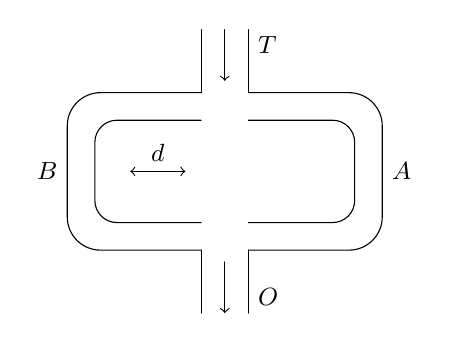
\begin{tikzpicture}[font=\small,line cap=round,line join=round]
\draw[rounded corners=12pt](-.3,1)--(-2,1)--(-2,-1)--(-.3,-1);\draw[rounded corners=8pt](-.3,.65)--(-1.65,.65)--(-1.65,-.65)--(-.3,-.65);\draw[rounded corners=12pt](.3,1)--(2,1)--(2,-1)--(.3,-1);\draw[rounded corners=8pt](.3,.65)--(1.65,.65)--(1.65,-.65)--(.3,-.65);\draw(-.3,1)--(-.3,1.8) (.3,1)--(.3,1.8) (-.3,-1)--(-.3,-1.8) (.3,-1)--(.3,-1.8);\draw[->](0,1.8)--(0,1.15);\draw[->](0,-1.15)--(0,-1.8);\node[right]at(.3,1.6){$T$};\node[right]at(.3,-1.6){$O$};\node[left]at(-2,0){$B$};\node[right]at(2,0){$A$};\draw[<->](-1.2,0)--node[above]{$d$}(-.5,0);
\end{tikzpicture}
